\chapter{Methodology and Design Process}

This chapter contains the design of the application architecture, the design of the scanning methodology and the description of the Agile method used to develop the application.

% •	Description of the application architecture suitable for security scanning (executable, terminal, later ui)
%%% o	System Settings UI and API to control every aspect of the device
% •	Agile method, stories, backlog

% IEC62443 findings and table
% Go language
% Explanation of the libraries used (Cobra for CLI, Zerolog for logging) and their benefits
% •	Design of the scanning methodology.
%%% o	Aspects covered: Outdated OS, outdated libraries (e.g., OpenSSL), outdated software, default or weak credentials, insecure network communication, …

\section{Agile method}

The \textit{Agile methodology} is a project management philosophy that involves breaking the project into phases and emphasizes continuous collaboration and improvement. Teams follow a cycle of planning, executing and evaluating. Teams choose agile so they can respond to changes in the marketplace or feedback from customers quickly without derailing a year's worth of plans. The publication of the Agile Manifesto\footnote{\url{https://agilemanifesto.org}} in 2001 marks the birth of agile as a methodology. Since then, many agile frameworks have emerged such as scrum, kanban or lean. Each embodies the core principles of frequent iteration, continuous learning and high quality in its own way.~\cite{agile-methodology} \\
We are now going to explain the Scrum framework, used by the company.

\subsection{Scrum}

Scrum is an agile project management framework, which is different from Agile, a philosophy.\\
The definition of scrum is based on empiricism and lean thinking. Empiricism says that knowledge comes from experience and that decisions are made based on what is observed. Lean thinking reduces waste and focuses on essentials. The scrum framework is heuristic; it is based on continuous learning and adjustment to fluctuating factors by acknowledging that the team does not know everything at the start of a project and it will evolve through experience. Scrum is structured to help teams to naturally adapt to changing conditions and user requirements, with re-prioritization built into the process and short release cycles so your team can constantly learn and improve.~\cite{scrum}

Scrum artefacts help to define the product, what work has to be done to create it and who has to do it. An \textit{epic} is a large body of work that can be broken down into smaller tasks. Each of these tasks is called \textit{story} and it is a short requirement written from the perspective of an end user. The story is linked to a person in the team that has to carry it out.

The two main artefacts boards are the \textit{product backlog} and the \textit{sprint backlog}. \\
The former is a list of all the tasks that needs to be done; it is a dynamic list of features, requirements, improvements, fixes and epics, ordered by their priority. Essentially, it is a \textit{"To Do"} list.\\
The latter is a list of items selected for the current sprint cycle; the sprint cycle is a fixed period of time, usually up to four weeks. Before each sprint, the team selects items from the product backlog to work on. Epics are broken down into stories and stories are moved from the product backlog to the sprint backlog.~\cite{scrum-epic-stories}

\begin{figure}[t]
  \centering
  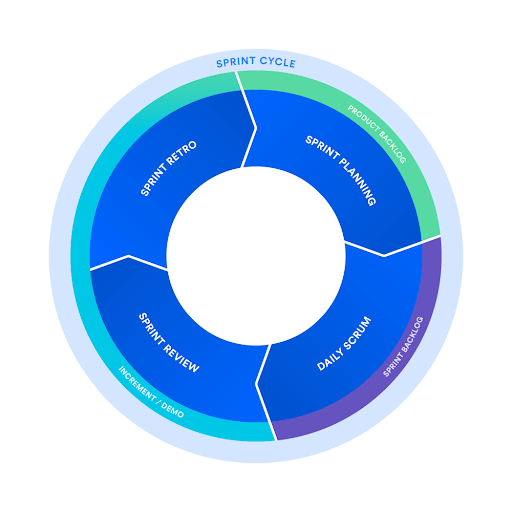
\includegraphics[width=0.8\textwidth]{chapters/04/assets/scrum}
  \caption{Scrum sprint cycle. Taken from \texttt{atlassian.com}}
  \label{fig:scrum-sprint-cycle}
\end{figure}

As visible in~\cref{fig:scrum-sprint-cycle}, Scrum is split in four principal phases:
\begin{itemize}
  \item The \textbf{sprint planning} is the initial phase of a sprint, the actual time period when the scrum team works; the team meets and decides what to do in the sprint by placing the tasks from the product backlog to the sprint backlog;
  \item The \textbf{daily scrum} is a quotidian meeting where the team members synchronize with each other. It is usually taken stand-up, as a way to not waste time and to keep the meeting short;
  \item The \textbf{sprint review} and \textbf{sprint retrospective} are the meetings at the end of the sprint where the team shows what they have done and demonstrates the work to the stakeholders and receive feedback;
\end{itemize}

The company takes advantage of the Scrum framework to manage the development of the cloud software, via the \textit{Jira} suite\footnote{\url{https://www.atlassian.com/software/jira}}, a project management tool developed by Atlassian. The platform is used to manage the product and the sprint backlog, the epics and the stories and to track the progress of the team.

% TODO: Descrivere board di Jira, colonne, priorità

Given that we were part of the office team, together with the business tutor we created a new Epic for the scanning tool and we filled it with the stories that we thought were needed to develop the tool. In this specific case, the sprint period was two months because of the internship duration. At the end of the sprint, the product backlog contained some pending stories, because of the limited time and the ongoing updating of the priorities. The daily scrum was achieved by a quotidian quick meeting with the business tutor, where we keep him updated on the progress of the stories. Of course, new stories were added to the backlog and some of them were de-prioritized.


\section{How IEC 62443 has driven the design}
\label{sec:iec-62443-driven-design}

Recalling~\cref{sec:iec-62443}, the IEC 62443 standard provides a comprehensive framework for securing industrial control systems and operational technology networks. In order to perform a step towards the certification of the devices with the standard, the scanning tool must cover at least the aspects of the standard.

We did a case study on the standard documentation: for each of the security requirements listed in the \texttt{3-3}, \texttt{4-1} and \texttt{4-2} documents, we said:
\begin{mdframed}
  \textit{\textless\textless  Can we implement a check for this requirement in such a way as to make the user able to fix the potential issue by itself? \textgreater\textgreater}
\end{mdframed}
We considered the user as a person that has a management account on the device, and that has to interact using the settings web interface. The goal was to make the final user able to fix the reported issue without the need to update the firmware or ask for a modification on the source code or on the development lifecycle by reporting a bug report.

\cref{fig:iec62443-findings-3_3} and~\cref{fig:iec62443-findings-4_2} show the findings of the case-study. The table is divided into four columns: the first one is the security requirement title, the second one is the description text, the third is whether we believe that it is a check we should implement on a scanning tool and the fourth one contains some notes about the possible implementation.

\begin{figure}[t]
  \centering
  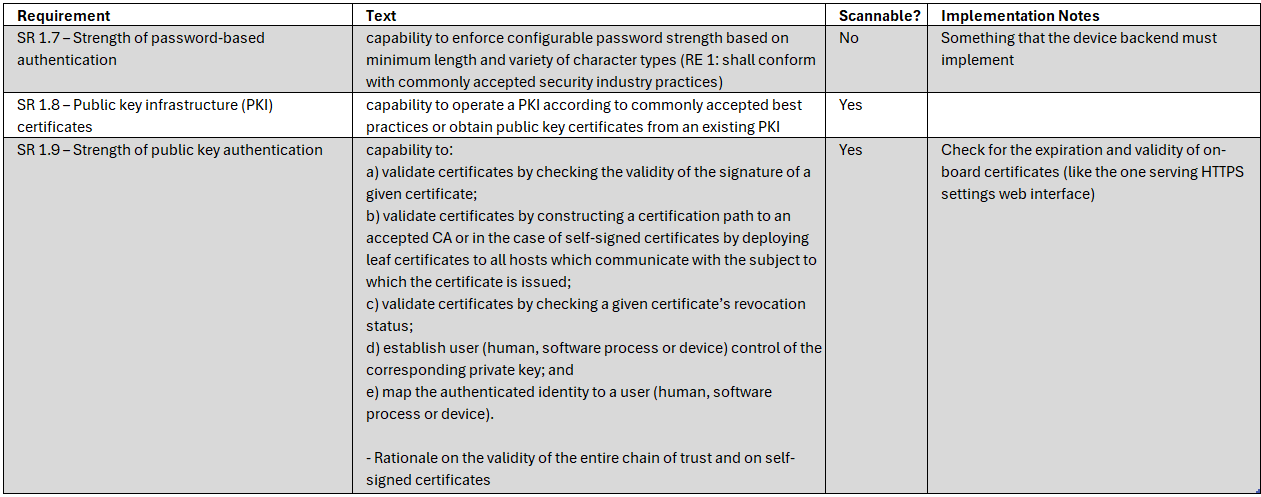
\includegraphics[width=1.0\textwidth]{chapters/04/assets/iec62443-findings-3_3}
  \caption{IEC 62443 \texttt{3-3} chosen requirements}
  \label{fig:iec62443-findings-3_3}
\end{figure}

\begin{figure}[t]
  \centering
  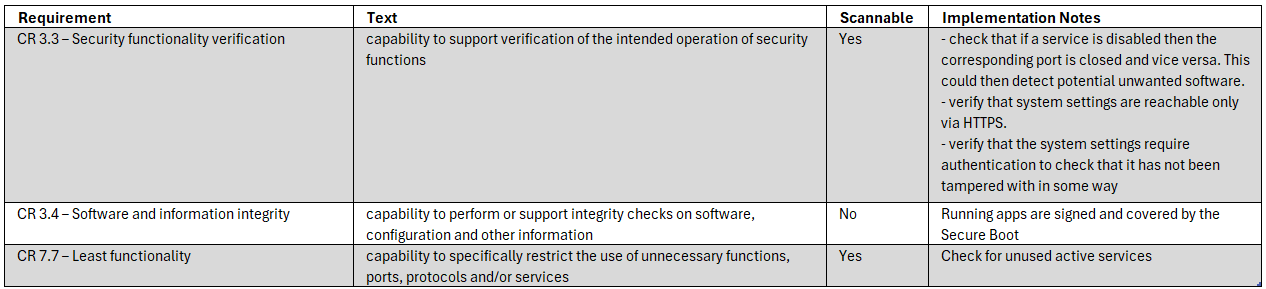
\includegraphics[width=1.0\textwidth]{chapters/04/assets/iec62443-findings-4_2}
  \caption{IEC 62443 \texttt{4-2} chosen requirements}
  \label{fig:iec62443-findings-4_2}
\end{figure}

To better explain our choices and motivations, we now take into account the \textit{SR 1.9 - Strength of public key authentication} requirement. The requirement states that there must be the capability to validate the validity of the used certificates by checking the signature, the expiration date and the revocation status. We believe that this is a check that we should implement in the scanning tool because the user can fix the issue by itself by renewing the certificate, or by changing the certificate authority related to it if needed. The implementation of the check could be done by retrieving the certificate from the device and then checking the signature, the expiration date and the revocation status. If the certificate is self-signed, the tool could suggest the user to change it with a certificate signed by a trusted certificate authority.

Instead, we now consider the \textit{SR 1.7 - Strength of password-based authentication}. The requirement states that the password must have a minimum length and a variety of character types. We put this assertion in a limbo, because if the user can set a password not respecting the requirement, the tool, which is a read-only intermediate between the user and the backend, cannot enforce the requirement. Then, the issue should be solved by the R\&D team, which should implement a password policy on the backend, and the user should be forced to change the password at the next login.

With this approach, we have identified the checks that the scanning tool should cover for sure from the standard and we have included them in the backlog of the project.

\section{Backlog stories}

With the help of the supervisor, we created a backlog of stories for the scanning tool. We drafted a new epic on the board and we filled it with the stories that we thought were needed to develop the tool.

We considered each story as an independent task that could be developed and tested in a short time, usually in a week. So, we split the epic into small stories, each one with a title, a description and a priority.

We started from the basis of a software, so the first stories were about the setup of the project and the thinking about the working architecture, the required parameters and the output formatting of the CLI. We want to keep the functioning of the tool as simple as possible and as much universal and reusable as possible. As a reference, we took inspiration by the help pages of some common softwares like \texttt{npm}, the node package manager, or \texttt{curl}, the tool to perform network requests directly on the terminal. Therefore, we sketched out the manual help page to have an overview of the commands and the options that the user could use.

At first glance, we decided to implement the following flow: the user runs the tool with the \texttt{scan} command, then the tool retrieves the device settings and the network status, then it performs the checks and finally it outputs the results to the console. The user can otherwise choose to save the output as a external file. The flag \texttt{--verbose} can be used to print more information about the checks and the results. The flag \texttt{--help} can be used to print the manual page or to print the documentation for a specific command.

The scan with no further options should perform all the checks that the tool can do as a default option, while the user can choose to perform only a subset of the checks by opting-in using the \texttt{--list} flag. The list of the available checks is available issuing the \texttt{list} command.

\begin{lstlisting}[caption={Man page}]
$ ./scantool
Industrial Security Scanning

Usage:
  scantool [command]

Available Commands:
  completion  Generate the autocompletion script for the specified shell
  help        Help about any command
  list        Show all the available scans
  scan        Start the device scan (options available typing `scan --help`)
  version     Print the version number

Flags:
  -h, --help      help for ciss
  --verbose       Log developer messages on stdout
  -v, --version   version for ciss
\end{lstlisting}

Moreover, we thought that the tool should be able to perform a scan in every network condition, to not exclude a priori a customer with an offline configuration or with a network that does not allow outcoming connections. Therefore, we decided to implement two different modes: the online mode where the tool can reach the cloud to determine the latest available version of the softwares, and the offline mode where the tool cannot reach the cloud and it has to rely on the local timestamp supplied by some of the softwares and libraries. \\
From the board side, for each of the check that the tool should perform, we put at least two different stories, respectively one for the online mode and one for the offline mode.

Then, we sketched out the stories about the checks to perform, starting from those extracted from the IEC 62443 standard, as explained in~\cref{sec:iec-62443-driven-design}, but also adding some other checks that we thought were needed to be performed. We also added some stories about the cross-compilation of the tool, the logging library to use and the CLI library to use.

At this point, we have a rich backlog of stories that we can work on and that we can prioritize according to the needs of the company.

The following list shows the stories that we have drafted for the scanning tool at the beginning of the project:
\begin{itemize}
  \item Choose a CLI library
  \item Choose a logging library
  \item Split flow into offline and online usage
  \item Check correct time
  \item JSON output
  \item Cross build script
  \item Scan OS version - date based
  \item Scan OS version - version based
  \item Default BSP user credentials
  \item Default BSP admin credentials
  \item Scan SSH port
  \item Check VNC credentials
  \item Check certificate expiration
  \item Verbose flag
  \item Add YAML report formatter
\end{itemize}

The list is not exhaustive and it is subject to changes during the development of the tool. It is ranked by a first look at the priority of the stories, but the priority can change during the advancement of the project.

\section{Choosing the libraries}

Starting from the scratch, we have to take care at first point of some utility libraries that we can use to draft the basis to develop the tool: we have to choose a CLI library to interact with and parse the command-line arguments, and a logging library to show the debug messages on the console or in another location.

\subsection{CLI library}

The comparison for the CLI parameters parsing is between a library called \textit{urfave/cli/v2}\footnote{\url{https://github.com/urfave/cli}} (\texttt{v2.27.1}) and another one called \textit{spf13/cobra}\footnote{\url{https://github.com/spf13/cobra}} (\texttt{v1.8.0}). Data and evaluation refers to March 2024.

Both the libraries have been suggested by the supervisor, and they are both widely used in the Go community. The evaluation between the two libraries is based on the features that they offer, the ease of use and the community support. In particular, we are interested in the ability to define flags and arguments, the ability to define commands and subcommands, the complexity to have the help page or the version of the tool.\\
Flags and arguments are the parameters that the user can pass to the tool to modify its behaviour, while commands are the different actions that the tool can perform. For example, the \texttt{scan} command is a command, while \texttt{--verbose} is a flag. Flag could be global, meaning that can be issued with every other command, or local, meaning that it has to be recognized only after a specified command or argument. A pattern to follow is \texttt{APPNAME COMMAND ARG --FLAG}. Finally, it's not obvious that a library supports the \textit{context} parameter, that is a way to pass data between the functions accross the application.

\textit{urfave/cli/v2} is a package for building command line apps in Go. The package provides a way to define flags and arguments, and it also provides a way to define commands. The package has a friendly documentation and it is actively maintained by the contributors. It is quick to define the actions for each flag or option. It supports the \textit{context} parameter. There is an upcoming major version \texttt{v3} in development, but it is not yet documented at all. The package has 21k stars on GitHub.

\textit{spf13/cobra} is an alike package for building command line apps in Go. The package provides a way to define flags and arguments, and it also provides a way to define commands. The documentation points directly to the source code, which is less friendly than the other package but anyway it is very rich and always updated. It supports the ability to deprecate a flag or a command with a custom message. It supports the \textit{context} parameter and an intelligent system of suggestions on typos, for example if the user types a command that does not exist, the package suggests the most similar command. The package has 35k stars on GitHub and it is actively maintained.

We initialized an empty project and we tried to implement the same simple CLI with both the libraries, one at time. The build size on the development laptop architecture with the first library was 4.8MB; with the second package was 5.1MB. The same working draft required 96 lines of code for the former and 110 lines of code for the latter.

In the end, we decided to use the \textit{spf13/cobra} because of the upcoming major version of \textit{cli/v2} which we do not know whether it will contain breaking changes or not, because the nice feature to deprecate an option, which could be useful given the youth of the project and possible future changes to the command-line interface and because of the capability to suggest the most similar command in case of a typo. The build size and the lines of code to get the same result are negligible for the use case of the tool.

\subsection{Log library}

The comparison for the logging library is between the standard library \textit{log}\footnote{\url{https://pkg.go.dev/log}} and another one called \textit{rs/zerolog}\footnote{\url{https://github.com/rs/zerolog}} (\texttt{v1.32.0}). Data and evaluation refers to April 2024.

The standard library \texttt{log} is the default logging package in Go. It provides a simple way to log messages with methods for formatting output. The package is easy to use and it is well documented. It supports the ability to log messages with different levels of severity, like \texttt{Info}, \texttt{Warning} and \texttt{Error}. The package is actively maintained by the contributors.

The \textit{rs/zerolog} lib, standing for \textit{Zero Allocation JSON Logger}, is another package for logging messages in Go. The package provides a way to log messages to the console or to a file. It also supports the different severity levels. The authors claim that the package is faster than other libraries because it does not allocate memory for the log messages~\cite{go-zerolog-benchmarks}. Furthermore, it implements a pretty logging, a way to format the output in a human-readable way, the hooks to attach custom functions on an event, the \textit{context} integration and much more. It is actively maintained and it has 10k stars on GitHub.

With all being said, we decided to use the \textit{rs/zerolog} library because of the performance and the features that it offers. The package was also already used by the company in the cloud software, so it was a good choice to keep the same library for the scanning tool.

\section{Platform applications}

The cloud management platform has an applications store where the developers can upload their \textit{apps}.

The scaffolding of the app is provided by a public NPM package. It is a drafted working application, so the developer can start to develop the app without the need to set up the project from scratch. Furthermore, it contains the necessary base configuration files to deploy the app to the platform. The app has to be deployed in a dedicated Kubernetes namespace in a cluster, and later it has to be pushed to the app store by using the public platform APIs.

An scaffolding app is composed of two layer: the frontend, which is the user interface, and the backend, which is the logic of the application. The frontend is written in VueJS\footnote{\url{https://vuejs.org}} and the backend is written in NestJS\footnote{\url{https://nestjs.com}}, a progressive Node.js framework. The former is a web application that the user can access from the cloud platform and the latter manages REST APIs.

\subsection{Scanning tool app}

The scanning tool is a command-line interface (CLI) application written in Go. The tool is designed to be run on the terminal of the device, so it can be used by the user to check the configuration of the device. As an initial idea, the tool should be able to perform a scan of the device and to output the results to the console. Thinking about the future, the scanning tool should be able to be run periodically and report the results to a central server, so the user can have a dashboard with the status of all the devices.

The idea to consider is to upload the scanning tool to the apps store, so the user can enable the wider automated view directly from the platform; doing so, the customer can create a campaign to check the configuration of all the devices from the same place and receive aggregated reports, with the goal to have a centralized view of the security status of the devices.

% As a educational project during the internship, we also have to develop the platform app for the scanning tool. We effectively setup the backend to be used as a proxy, and the frontend is a simple page that 
